  

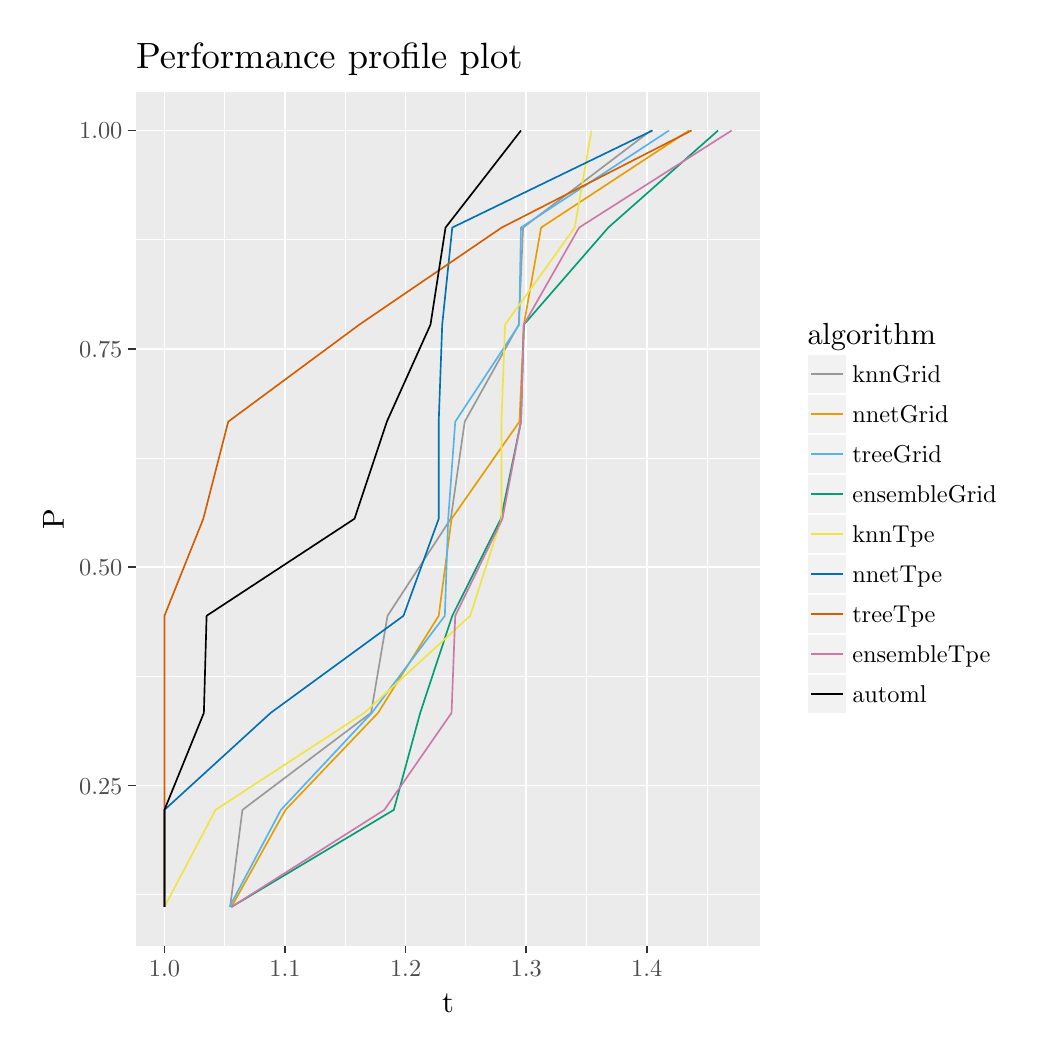
\begin{tikzpicture}[x=1pt,y=1pt]
\definecolor{fillColor}{RGB}{255,255,255}
\path[use as bounding box,fill=fillColor,fill opacity=0.00] (0,0) rectangle (361.35,361.35);
\begin{scope}
\path[clip] (  0.00,  0.00) rectangle (361.35,361.35);
\definecolor{drawColor}{RGB}{255,255,255}
\definecolor{fillColor}{RGB}{255,255,255}

\path[draw=drawColor,line width= 0.6pt,line join=round,line cap=round,fill=fillColor] (  0.00,  0.00) rectangle (361.35,361.35);
\end{scope}
\begin{scope}
\path[clip] ( 39.17, 29.59) rectangle (264.64,338.21);
\definecolor{fillColor}{gray}{0.92}

\path[fill=fillColor] ( 39.17, 29.59) rectangle (264.64,338.21);
\definecolor{drawColor}{RGB}{255,255,255}

\path[draw=drawColor,line width= 0.3pt,line join=round] ( 39.17, 48.00) --
	(264.64, 48.00);

\path[draw=drawColor,line width= 0.3pt,line join=round] ( 39.17,126.91) --
	(264.64,126.91);

\path[draw=drawColor,line width= 0.3pt,line join=round] ( 39.17,205.82) --
	(264.64,205.82);

\path[draw=drawColor,line width= 0.3pt,line join=round] ( 39.17,284.73) --
	(264.64,284.73);

\path[draw=drawColor,line width= 0.3pt,line join=round] ( 71.20, 29.59) --
	( 71.20,338.21);

\path[draw=drawColor,line width= 0.3pt,line join=round] (114.78, 29.59) --
	(114.78,338.21);

\path[draw=drawColor,line width= 0.3pt,line join=round] (158.35, 29.59) --
	(158.35,338.21);

\path[draw=drawColor,line width= 0.3pt,line join=round] (201.93, 29.59) --
	(201.93,338.21);

\path[draw=drawColor,line width= 0.3pt,line join=round] (245.51, 29.59) --
	(245.51,338.21);

\path[draw=drawColor,line width= 0.6pt,line join=round] ( 39.17, 87.45) --
	(264.64, 87.45);

\path[draw=drawColor,line width= 0.6pt,line join=round] ( 39.17,166.37) --
	(264.64,166.37);

\path[draw=drawColor,line width= 0.6pt,line join=round] ( 39.17,245.28) --
	(264.64,245.28);

\path[draw=drawColor,line width= 0.6pt,line join=round] ( 39.17,324.19) --
	(264.64,324.19);

\path[draw=drawColor,line width= 0.6pt,line join=round] ( 49.42, 29.59) --
	( 49.42,338.21);

\path[draw=drawColor,line width= 0.6pt,line join=round] ( 92.99, 29.59) --
	( 92.99,338.21);

\path[draw=drawColor,line width= 0.6pt,line join=round] (136.57, 29.59) --
	(136.57,338.21);

\path[draw=drawColor,line width= 0.6pt,line join=round] (180.14, 29.59) --
	(180.14,338.21);

\path[draw=drawColor,line width= 0.6pt,line join=round] (223.72, 29.59) --
	(223.72,338.21);
\definecolor{drawColor}{gray}{0.60}

\path[draw=drawColor,line width= 0.6pt,line join=round] ( 73.16, 43.62) --
	( 77.59, 78.69) --
	(124.08,113.76) --
	(130.03,148.83) --
	(152.90,183.90) --
	(157.92,218.97) --
	(177.45,254.04) --
	(179.01,289.11) --
	(225.22,324.19);
\definecolor{drawColor}{RGB}{230,159,0}

\path[draw=drawColor,line width= 0.6pt,line join=round] ( 73.62, 43.62) --
	( 93.15, 78.69) --
	(126.62,113.76) --
	(148.53,148.83) --
	(153.17,183.90) --
	(177.70,218.97) --
	(179.29,254.04) --
	(185.53,289.11) --
	(238.99,324.19);
\definecolor{drawColor}{RGB}{86,180,233}

\path[draw=drawColor,line width= 0.6pt,line join=round] ( 72.93, 43.62) --
	( 91.50, 78.69) --
	(124.36,113.76) --
	(150.74,148.83) --
	(151.95,183.90) --
	(154.50,218.97) --
	(177.60,254.04) --
	(178.25,289.11) --
	(231.75,324.19);
\definecolor{drawColor}{RGB}{0,158,115}

\path[draw=drawColor,line width= 0.6pt,line join=round] ( 73.62, 43.62) --
	(132.30, 78.69) --
	(141.84,113.76) --
	(153.43,148.83) --
	(171.01,183.90) --
	(178.25,218.97) --
	(179.29,254.04) --
	(209.80,289.11) --
	(249.48,324.19);
\definecolor{drawColor}{RGB}{240,228,66}

\path[draw=drawColor,line width= 0.6pt,line join=round] ( 49.42, 43.62) --
	( 67.87, 78.69) --
	(121.65,113.76) --
	(159.90,148.83) --
	(171.19,183.90) --
	(171.19,218.97) --
	(172.50,254.04) --
	(197.67,289.11) --
	(203.73,324.19);
\definecolor{drawColor}{RGB}{0,114,178}

\path[draw=drawColor,line width= 0.6pt,line join=round] ( 49.42, 43.62) --
	( 49.42, 78.69) --
	( 87.82,113.76) --
	(135.80,148.83) --
	(148.53,183.90) --
	(148.53,218.97) --
	(149.79,254.04) --
	(153.43,289.11) --
	(225.78,324.19);
\definecolor{drawColor}{RGB}{213,94,0}

\path[draw=drawColor,line width= 0.6pt,line join=round] ( 49.42, 43.62) --
	( 49.42, 78.69) --
	( 49.42,113.76) --
	( 49.42,148.83) --
	( 63.47,183.90) --
	( 72.47,218.97) --
	(119.85,254.04) --
	(171.28,289.11) --
	(239.89,324.19);
\definecolor{drawColor}{RGB}{204,121,167}

\path[draw=drawColor,line width= 0.6pt,line join=round] ( 73.62, 43.62) --
	(128.87, 78.69) --
	(153.17,113.76) --
	(154.49,148.83) --
	(171.56,183.90) --
	(178.25,218.97) --
	(179.29,254.04) --
	(199.26,289.11) --
	(254.39,324.19);
\definecolor{drawColor}{RGB}{0,0,0}

\path[draw=drawColor,line width= 0.6pt,line join=round] ( 49.42, 43.62) --
	( 49.42, 78.69) --
	( 63.67,113.76) --
	( 64.65,148.83) --
	(118.10,183.90) --
	(129.78,218.97) --
	(145.56,254.04) --
	(150.99,289.11) --
	(178.25,324.19);
\end{scope}
\begin{scope}
\path[clip] (  0.00,  0.00) rectangle (361.35,361.35);
\definecolor{drawColor}{gray}{0.30}

\node[text=drawColor,anchor=base east,inner sep=0pt, outer sep=0pt, scale=  0.88] at ( 34.22, 84.42) {0.25};

\node[text=drawColor,anchor=base east,inner sep=0pt, outer sep=0pt, scale=  0.88] at ( 34.22,163.33) {0.50};

\node[text=drawColor,anchor=base east,inner sep=0pt, outer sep=0pt, scale=  0.88] at ( 34.22,242.25) {0.75};

\node[text=drawColor,anchor=base east,inner sep=0pt, outer sep=0pt, scale=  0.88] at ( 34.22,321.16) {1.00};
\end{scope}
\begin{scope}
\path[clip] (  0.00,  0.00) rectangle (361.35,361.35);
\definecolor{drawColor}{gray}{0.20}

\path[draw=drawColor,line width= 0.6pt,line join=round] ( 36.42, 87.45) --
	( 39.17, 87.45);

\path[draw=drawColor,line width= 0.6pt,line join=round] ( 36.42,166.37) --
	( 39.17,166.37);

\path[draw=drawColor,line width= 0.6pt,line join=round] ( 36.42,245.28) --
	( 39.17,245.28);

\path[draw=drawColor,line width= 0.6pt,line join=round] ( 36.42,324.19) --
	( 39.17,324.19);
\end{scope}
\begin{scope}
\path[clip] (  0.00,  0.00) rectangle (361.35,361.35);
\definecolor{drawColor}{gray}{0.20}

\path[draw=drawColor,line width= 0.6pt,line join=round] ( 49.42, 26.84) --
	( 49.42, 29.59);

\path[draw=drawColor,line width= 0.6pt,line join=round] ( 92.99, 26.84) --
	( 92.99, 29.59);

\path[draw=drawColor,line width= 0.6pt,line join=round] (136.57, 26.84) --
	(136.57, 29.59);

\path[draw=drawColor,line width= 0.6pt,line join=round] (180.14, 26.84) --
	(180.14, 29.59);

\path[draw=drawColor,line width= 0.6pt,line join=round] (223.72, 26.84) --
	(223.72, 29.59);
\end{scope}
\begin{scope}
\path[clip] (  0.00,  0.00) rectangle (361.35,361.35);
\definecolor{drawColor}{gray}{0.30}

\node[text=drawColor,anchor=base,inner sep=0pt, outer sep=0pt, scale=  0.88] at ( 49.42, 18.58) {1.0};

\node[text=drawColor,anchor=base,inner sep=0pt, outer sep=0pt, scale=  0.88] at ( 92.99, 18.58) {1.1};

\node[text=drawColor,anchor=base,inner sep=0pt, outer sep=0pt, scale=  0.88] at (136.57, 18.58) {1.2};

\node[text=drawColor,anchor=base,inner sep=0pt, outer sep=0pt, scale=  0.88] at (180.14, 18.58) {1.3};

\node[text=drawColor,anchor=base,inner sep=0pt, outer sep=0pt, scale=  0.88] at (223.72, 18.58) {1.4};
\end{scope}
\begin{scope}
\path[clip] (  0.00,  0.00) rectangle (361.35,361.35);
\definecolor{drawColor}{RGB}{0,0,0}

\node[text=drawColor,anchor=base,inner sep=0pt, outer sep=0pt, scale=  1.10] at (151.90,  5.50) {t};
\end{scope}
\begin{scope}
\path[clip] (  0.00,  0.00) rectangle (361.35,361.35);
\definecolor{drawColor}{RGB}{0,0,0}

\node[text=drawColor,rotate= 90.00,anchor=base,inner sep=0pt, outer sep=0pt, scale=  1.10] at ( 13.08,183.90) {P};
\end{scope}
\begin{scope}
\path[clip] (  0.00,  0.00) rectangle (361.35,361.35);
\definecolor{fillColor}{RGB}{255,255,255}

\path[fill=fillColor] (276.02,107.57) rectangle (355.85,260.23);
\end{scope}
\begin{scope}
\path[clip] (  0.00,  0.00) rectangle (361.35,361.35);
\definecolor{drawColor}{RGB}{0,0,0}

\node[text=drawColor,anchor=base west,inner sep=0pt, outer sep=0pt, scale=  1.10] at (281.71,246.96) {algorithm};
\end{scope}
\begin{scope}
\path[clip] (  0.00,  0.00) rectangle (361.35,361.35);
\definecolor{drawColor}{RGB}{255,255,255}
\definecolor{fillColor}{gray}{0.95}

\path[draw=drawColor,line width= 0.6pt,line join=round,line cap=round,fill=fillColor] (281.71,228.90) rectangle (296.16,243.35);
\end{scope}
\begin{scope}
\path[clip] (  0.00,  0.00) rectangle (361.35,361.35);
\definecolor{drawColor}{gray}{0.60}

\path[draw=drawColor,line width= 0.6pt,line join=round] (283.16,236.12) -- (294.72,236.12);
\end{scope}
\begin{scope}
\path[clip] (  0.00,  0.00) rectangle (361.35,361.35);
\definecolor{drawColor}{RGB}{255,255,255}
\definecolor{fillColor}{gray}{0.95}

\path[draw=drawColor,line width= 0.6pt,line join=round,line cap=round,fill=fillColor] (281.71,214.44) rectangle (296.16,228.90);
\end{scope}
\begin{scope}
\path[clip] (  0.00,  0.00) rectangle (361.35,361.35);
\definecolor{drawColor}{RGB}{230,159,0}

\path[draw=drawColor,line width= 0.6pt,line join=round] (283.16,221.67) -- (294.72,221.67);
\end{scope}
\begin{scope}
\path[clip] (  0.00,  0.00) rectangle (361.35,361.35);
\definecolor{drawColor}{RGB}{255,255,255}
\definecolor{fillColor}{gray}{0.95}

\path[draw=drawColor,line width= 0.6pt,line join=round,line cap=round,fill=fillColor] (281.71,199.99) rectangle (296.16,214.44);
\end{scope}
\begin{scope}
\path[clip] (  0.00,  0.00) rectangle (361.35,361.35);
\definecolor{drawColor}{RGB}{86,180,233}

\path[draw=drawColor,line width= 0.6pt,line join=round] (283.16,207.21) -- (294.72,207.21);
\end{scope}
\begin{scope}
\path[clip] (  0.00,  0.00) rectangle (361.35,361.35);
\definecolor{drawColor}{RGB}{255,255,255}
\definecolor{fillColor}{gray}{0.95}

\path[draw=drawColor,line width= 0.6pt,line join=round,line cap=round,fill=fillColor] (281.71,185.53) rectangle (296.16,199.99);
\end{scope}
\begin{scope}
\path[clip] (  0.00,  0.00) rectangle (361.35,361.35);
\definecolor{drawColor}{RGB}{0,158,115}

\path[draw=drawColor,line width= 0.6pt,line join=round] (283.16,192.76) -- (294.72,192.76);
\end{scope}
\begin{scope}
\path[clip] (  0.00,  0.00) rectangle (361.35,361.35);
\definecolor{drawColor}{RGB}{255,255,255}
\definecolor{fillColor}{gray}{0.95}

\path[draw=drawColor,line width= 0.6pt,line join=round,line cap=round,fill=fillColor] (281.71,171.08) rectangle (296.16,185.53);
\end{scope}
\begin{scope}
\path[clip] (  0.00,  0.00) rectangle (361.35,361.35);
\definecolor{drawColor}{RGB}{240,228,66}

\path[draw=drawColor,line width= 0.6pt,line join=round] (283.16,178.31) -- (294.72,178.31);
\end{scope}
\begin{scope}
\path[clip] (  0.00,  0.00) rectangle (361.35,361.35);
\definecolor{drawColor}{RGB}{255,255,255}
\definecolor{fillColor}{gray}{0.95}

\path[draw=drawColor,line width= 0.6pt,line join=round,line cap=round,fill=fillColor] (281.71,156.63) rectangle (296.16,171.08);
\end{scope}
\begin{scope}
\path[clip] (  0.00,  0.00) rectangle (361.35,361.35);
\definecolor{drawColor}{RGB}{0,114,178}

\path[draw=drawColor,line width= 0.6pt,line join=round] (283.16,163.85) -- (294.72,163.85);
\end{scope}
\begin{scope}
\path[clip] (  0.00,  0.00) rectangle (361.35,361.35);
\definecolor{drawColor}{RGB}{255,255,255}
\definecolor{fillColor}{gray}{0.95}

\path[draw=drawColor,line width= 0.6pt,line join=round,line cap=round,fill=fillColor] (281.71,142.17) rectangle (296.16,156.63);
\end{scope}
\begin{scope}
\path[clip] (  0.00,  0.00) rectangle (361.35,361.35);
\definecolor{drawColor}{RGB}{213,94,0}

\path[draw=drawColor,line width= 0.6pt,line join=round] (283.16,149.40) -- (294.72,149.40);
\end{scope}
\begin{scope}
\path[clip] (  0.00,  0.00) rectangle (361.35,361.35);
\definecolor{drawColor}{RGB}{255,255,255}
\definecolor{fillColor}{gray}{0.95}

\path[draw=drawColor,line width= 0.6pt,line join=round,line cap=round,fill=fillColor] (281.71,127.72) rectangle (296.16,142.17);
\end{scope}
\begin{scope}
\path[clip] (  0.00,  0.00) rectangle (361.35,361.35);
\definecolor{drawColor}{RGB}{204,121,167}

\path[draw=drawColor,line width= 0.6pt,line join=round] (283.16,134.94) -- (294.72,134.94);
\end{scope}
\begin{scope}
\path[clip] (  0.00,  0.00) rectangle (361.35,361.35);
\definecolor{drawColor}{RGB}{255,255,255}
\definecolor{fillColor}{gray}{0.95}

\path[draw=drawColor,line width= 0.6pt,line join=round,line cap=round,fill=fillColor] (281.71,113.26) rectangle (296.16,127.72);
\end{scope}
\begin{scope}
\path[clip] (  0.00,  0.00) rectangle (361.35,361.35);
\definecolor{drawColor}{RGB}{0,0,0}

\path[draw=drawColor,line width= 0.6pt,line join=round] (283.16,120.49) -- (294.72,120.49);
\end{scope}
\begin{scope}
\path[clip] (  0.00,  0.00) rectangle (361.35,361.35);
\definecolor{drawColor}{RGB}{0,0,0}

\node[text=drawColor,anchor=base west,inner sep=0pt, outer sep=0pt, scale=  0.88] at (297.97,233.09) {knnGrid};
\end{scope}
\begin{scope}
\path[clip] (  0.00,  0.00) rectangle (361.35,361.35);
\definecolor{drawColor}{RGB}{0,0,0}

\node[text=drawColor,anchor=base west,inner sep=0pt, outer sep=0pt, scale=  0.88] at (297.97,218.64) {nnetGrid};
\end{scope}
\begin{scope}
\path[clip] (  0.00,  0.00) rectangle (361.35,361.35);
\definecolor{drawColor}{RGB}{0,0,0}

\node[text=drawColor,anchor=base west,inner sep=0pt, outer sep=0pt, scale=  0.88] at (297.97,204.18) {treeGrid};
\end{scope}
\begin{scope}
\path[clip] (  0.00,  0.00) rectangle (361.35,361.35);
\definecolor{drawColor}{RGB}{0,0,0}

\node[text=drawColor,anchor=base west,inner sep=0pt, outer sep=0pt, scale=  0.88] at (297.97,189.73) {ensembleGrid};
\end{scope}
\begin{scope}
\path[clip] (  0.00,  0.00) rectangle (361.35,361.35);
\definecolor{drawColor}{RGB}{0,0,0}

\node[text=drawColor,anchor=base west,inner sep=0pt, outer sep=0pt, scale=  0.88] at (297.97,175.28) {knnTpe};
\end{scope}
\begin{scope}
\path[clip] (  0.00,  0.00) rectangle (361.35,361.35);
\definecolor{drawColor}{RGB}{0,0,0}

\node[text=drawColor,anchor=base west,inner sep=0pt, outer sep=0pt, scale=  0.88] at (297.97,160.82) {nnetTpe};
\end{scope}
\begin{scope}
\path[clip] (  0.00,  0.00) rectangle (361.35,361.35);
\definecolor{drawColor}{RGB}{0,0,0}

\node[text=drawColor,anchor=base west,inner sep=0pt, outer sep=0pt, scale=  0.88] at (297.97,146.37) {treeTpe};
\end{scope}
\begin{scope}
\path[clip] (  0.00,  0.00) rectangle (361.35,361.35);
\definecolor{drawColor}{RGB}{0,0,0}

\node[text=drawColor,anchor=base west,inner sep=0pt, outer sep=0pt, scale=  0.88] at (297.97,131.91) {ensembleTpe};
\end{scope}
\begin{scope}
\path[clip] (  0.00,  0.00) rectangle (361.35,361.35);
\definecolor{drawColor}{RGB}{0,0,0}

\node[text=drawColor,anchor=base west,inner sep=0pt, outer sep=0pt, scale=  0.88] at (297.97,117.46) {automl};
\end{scope}
\begin{scope}
\path[clip] (  0.00,  0.00) rectangle (361.35,361.35);
\definecolor{drawColor}{RGB}{0,0,0}

\node[text=drawColor,anchor=base west,inner sep=0pt, outer sep=0pt, scale=  1.32] at ( 39.17,346.76) {Performance profile plot};
\end{scope}
\end{tikzpicture}


